
\section{Introduction}

\subsection{Aim and Scope} 

Work Package 3 (WP3) focuses on the design and development of ICT facilitation for social participation in the energy network to manage communities and support energy services. Deliverable 3.3 (D3.3) is described in the CIVIS project proposal as follows: 

\begin{quote}
D3.3) Final field tested Integrated Energy System: Output of T3.1-5; Based on information provided by the deployment of deliverable 3.2 the software is further refined to provide energy services and community management (open source). 
\end{quote}

The 3rd year's project activities continued the design and development of the software platform \textit{YouPower}\footnote{\url{http://civis.tbm.tudelft.nl/} or \url{https://app.civisproject.eu/}}, expanding upon the 2nd year's result reported in D3.2 \citep{Huang2015c}. 
As stated in D3.2, the CIVIS platform is composed of two parts (see Figure~\ref{fig:platform}): the services provided by the CIVIS back-end, and the CIVIS front-end application which users directly interact with. 
%
\begin{figure}[h!]
\begin{center}\footnotesize
	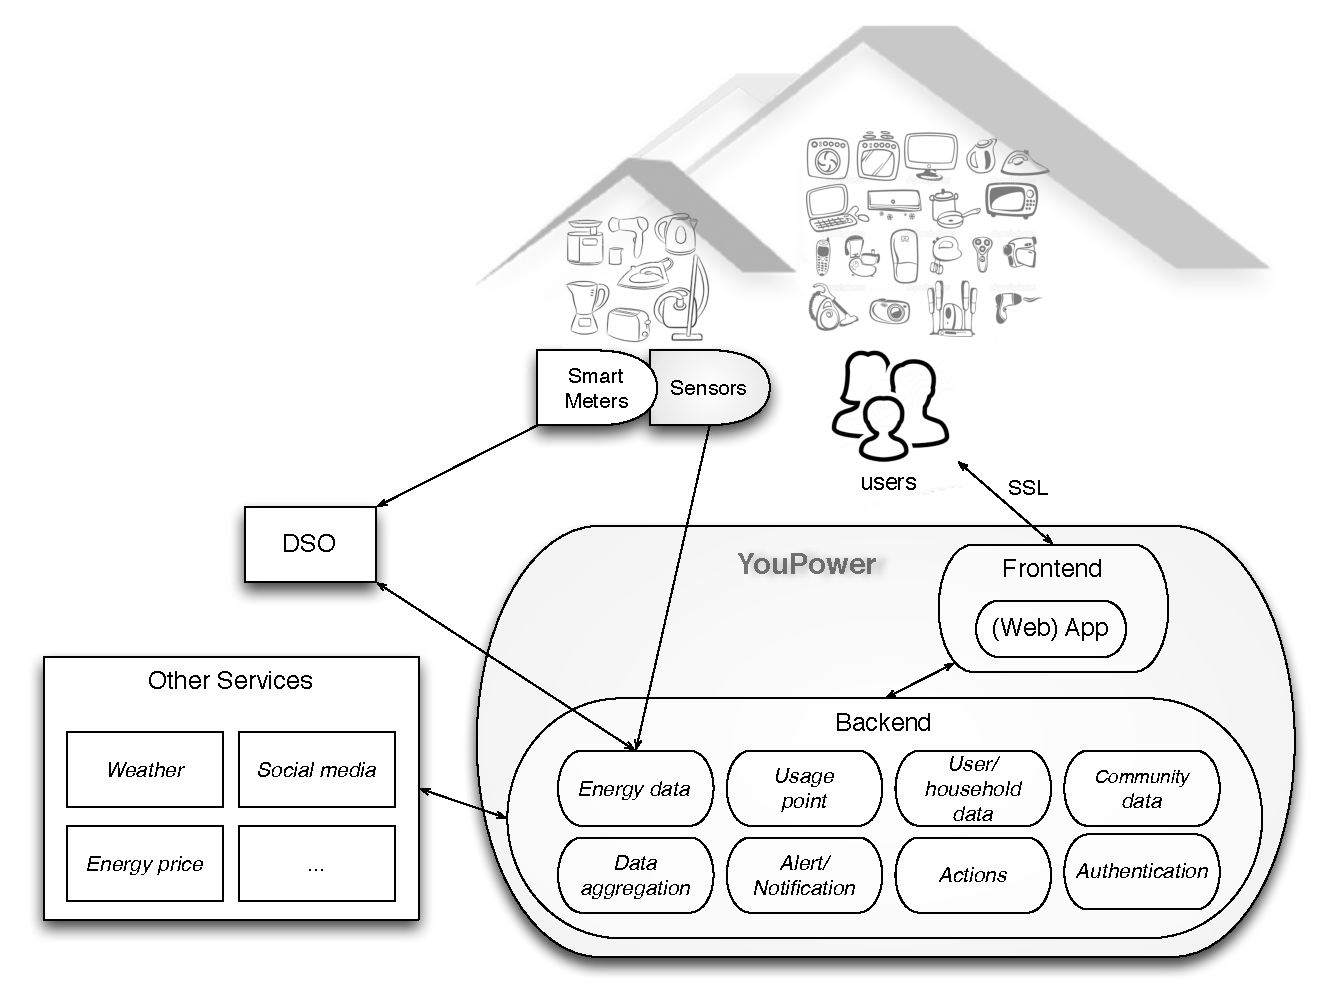
\includegraphics[width=.95\textwidth]{img/civis_platform_overview.pdf}\\
	DSO (Distribution System Operators),  SSL (Secure Sockets Layer)
	\caption{CIVIS platform overview}\label{fig:platform}
\end{center}
\end{figure}
% 
To this end, WP4 focuses on the system level ICT services that deal with the energy data and its collection through the smart meters and sensors installed at the Swedish and Italian test sites (see D4.3 for more details). 
% 
WP3 focuses on the front-end application and the social level ICT services that are related to users/prosumers, households, communities, energy consumptions, etc. 

In this report, we discuss the design and development of the WP3 part of the CIVIS platform known as YouPower\footnote{The CIVIS front-end application used to be called EnergyUP. The old name may be found in some old documents and/or mock-ups.}. 
The final results are summarized as a whole for readability and usefulness. The refinement and improvement made in the third year are highlighted where necessary when possible. 
% 
The functionalities of the platform reported are deployed at Stockholm (Sweden) and Trento (Italy) test sites respectively according to the local context. The YouPower software is open source under the Apache v.2 License\footnote{\url{https://github.com/CIVIS-project/YouPower/blob/master/LICENSE}}. It has  an online repository at GitHub\footnote{ \url{https://github.com/CIVIS-project/YouPower/}}. 
The backend API documentation is aslo available online\footnote{ \url{http://civis.tbm.tudelft.nl/apidoc/}}. 

%The authentication of user sign up and login to an EnergyUP account is managed by WP3 services. A user may also choose to link his or her energy data, additional authentication is required. 

\subsection{Design and Development: the Continuation}

Environmental problems have their origins in human behavoir; as a result, any solution to enviromental issues will require changes in behavoir 
\citep{Schultz2014}.
A novelty of the CIVIS project is that our research attention is geared towards the potentials and challenges of user's collective actions, pro-social values and sense of community. 
Collective human behavior is deemed critical because it is both a source and a solution to the problem of climate change \citep{Masson2014}.
In this context, the design of YouPower aims to support social participation, awareness and engagement by means of ICT in the smart grids to achieve sustainable energy goals such as consumption reduction and load shifting. We as researchers can also use this platform as a communication channel to promote sustainable energy goals, and as a research instrument to observe users' responses and possible outcomes. 

%The effectiveness of smart grids depends on consumer engagement and action. Today’s consumers have a vague understanding of the grid. 
%How consumers understand the smart grid will shape how they feel about it, and in turn how readily they adopt it, and how they use it. 
%If consumers are given useful feedback on how they use energy and are provided with recommendations on how to improve, they will have the chances to make more informed energy choices. 


The design and development of YouPower is theory-driven, user-centered and iterative \citep{Leffingwell2000,Leffingwell2011}. We extensively researched literature on intervention strategies and social smart grid applications directed at promoting pro environmental consumer behavior change. This provided an initial set of design ideas that are iteratively refined and improved through the design process. Applying a user-centered design process can lead to more acceptable, satisfying and effective designs \citep{Brynjarsdottir2012}. This increases the potential of the intervention \citep{dick2012empowering} and may help increase user engagement with respect to the sense of relatedness to the application \citep{pierce2003state,schwartz2014people,edward2015review}. 

In the 2nd year of CIVIS, we started with brainstorming sessions and a design workshop. A set of features was prototyped in simple handcrafted mock-ups used as a basis for discussion, and then underwent iterative rapid prototyping which produced wireframes as visual guides that can be more effectively communicated to general users. These prototypes were evaluated by user tests with groups of students and colleagues. Using the wireframe prototypes and later the software prototypes, we conducted focus group studies with consumers in Trento, test studies and focus groups with consumers and housing cooperative members in Stockholm, as well as a user study with pro-environmental participants in Helsinki. 

In the 3rd year of CIVIS, the iterative design and development process continued. We paid particular attention to quick responses to changes, user feedback and adaptive development. We also furthered literature research in environmental psychology and intervention design, and expanded the design guidelines based on literature, our design practices and experiences. These guidelines can be useful for a wider group of designers interested in pro-environmental information-based intervention. YouPower has been refined and improved gradually in the 3rd year resulting the current version of the application. The first deployment at the Stockholm test site was in Nov 2015 and Trento test site in Mar 2016 correspondingly. The production server (i.e. CIVIS YouPower server hosted by TU Delft) since then has been updated once there were new parts ready for deployment.  
The rest of this report presents and discusses the latest version of YouPower. 

%literature, group feedback (internal), user feedback: workshops, focus groups 
 
 

